\section{曲线的同伦·基本群}
\sourcepage{13--14}
本节介绍与曲线同伦概念有关的一些拓扑学结果。

拓扑空间$X$中的一条\textbf{曲线}是指连续映射$u:I\to X$，其中$I:=[0,1]\subset\R$为单位区间。点$a:=u(0)$称为$u$的起点，$b:=u(1)$称为终点。也称$u$为从$a$到$b$的曲线，或称曲线$u$连接$a$与$b$。

回顾：若拓扑空间$X$的任意两点$a,b$均可由曲线连接，则称$X$\textbf{弧连通}或\textbf{道路连通}（arcwise connected, pathwise connected）。弧连通空间也是连通的，即不存在$X=U_1\cup U_2$的分解，其中$U_1,U_2$为非空、不交的开集。若每一点都有由弧连通集组成的邻域基，则称空间局部弧连通。特别地，流形总满足这一条件。连通且局部弧连通的空间$X$是（整体）弧连通的，因为容易证明，所有能够与一个给定点$a\in X$用曲线连接的点$x\in X$组成的集合既开又闭。

\entry{3.1}{定义}
设$X$是拓扑空间，$a,b\in X$。称从$a$到$b$的两条曲线$u,v:I\to X$\textbf{同伦}（homotopic），记为$u\sim v$，如果存在连续映射$A:I\times I\to X$满足
\begin{enumerate}[label=(\roman*)]
\item 对每个$t\in I$，$A(t,0)=u(t)$；
\item 对每个$t\in I$，$A(t,1)=v(t)$；
\item 对每个$s\in I$，$A(0,s)=a$且$A(1,s)=b$。
\end{enumerate}
\textbf{注记。}若令$u_s(t):=A(t,s)$，则每个$u_s$都是从$a$到$b$的曲线，且$u_0=u$，$u_1=v$。曲线族$(u_s)_{0\le s\le1}$称为曲线$u$到曲线$v$的一个形变，或从$u$到$v$的一个同伦，参见图3。
\begin{center}\begin{minipage}{\linewidth}\centering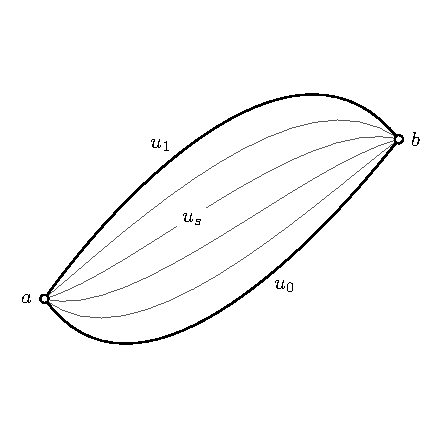
\includegraphics[width=.48\textwidth]{figures/fig03-tikz.pdf}\\图3\end{minipage}\end{center}
\entry{3.2}{定理}
设$X$是拓扑空间，$a,b\in X$。则同伦关系是从$a$到$b$的所有曲线组成的集合上的一个等价关系。
\begin{proof}
自反性和对称性显然。关于传递性，设$u,v,w:I\to X$是从$a$到$b$的三条曲线，且$u\sim v$、$v\sim w$。须证明$u\sim w$。
\sourcepage{15}
依假设，存在连续映射$A,B:I\times I\to X$，使对每个$t,s\in I$有
\begin{gather*}
A(t,0)=u(t),\quad A(t,1)=B(t,0)=v(t),\quad B(t,1)=w(t),\\
A(0,s)=B(0,s)=a,\quad A(1,s)=B(1,s)=b.
\end{gather*}
定义$C:I\times I\to X$为
\[
C(t,s):=\begin{cases}A(t,2s),&0\le s\le\tfrac12,\\B(t,2s-1),&\tfrac12\le s\le1.\end{cases}
\]
则$C$连续，是从$u$到$w$的同伦。
\end{proof}
\entry{3.3}{引理}
设$u:I\to X$是拓扑空间$X$中的曲线，$\varphi:I\to I$是满足$\varphi(0)=0$、$\varphi(1)=1$的连续映射。则曲线$u$和$u\circ\varphi$同伦。
\begin{proof}
定义$A:I\times I\to X$为$A(t,s):=u((1-s)t+s\varphi(t))$。则$A$连续，且对每个$t,s\in I$，
\[
A(t,0)=u(t),\quad A(t,1)=(u\circ\varphi)(t),\quad A(0,s)=u(0),\quad A(1,s)=u(1).
\]
因此$u$与$u\circ\varphi$同伦。
\end{proof}
\entry{3.4}{定义}
设$a,b,c$是拓扑空间$X$中的三点，$u:I\to X$是从$a$到$b$的曲线，$v:I\to X$是从$b$到$c$的曲线。

(i) 从$a$到$c$的\textbf{乘积曲线}$u\cdot v:I\to X$定义为
\[
(u\cdot v)(t):=\begin{cases}u(2t),&0\le t\le\tfrac12,\\v(2t-1),&\tfrac12\le t\le1.\end{cases}
\]
(ii) \textbf{逆曲线}$u^-:I\to X$定义为$u^-(t):=u(1-t)$（$t\in I$）。\translatornote{原文称逆曲线“从$a$到$b$”，但由定义其起点为$b$、终点为$a$。}

乘积曲线$u\cdot v$先经过曲线$u$上的点，再经过曲线$v$上的点，但速度均加倍。逆曲线$u^-$经过与$u$相同的点，方向相反。

容易验证，若$u_1,u_2:I\to X$为从$a$到$b$的同伦曲线，$v_1,v_2:I\to X$为从$b$到$c$的同伦曲线，则$u_1\cdot v_1\sim u_2\cdot v_2$，且$u_1^-\sim u_2^-$。
\sourcepage{16}
\entry{3.5}{定义}
设$X$是拓扑空间，$a\in X$。$a$处的\textbf{常曲线}是指常值映射$u_0:I\to X$，即对每个$t\in I$有$u_0(t)=a$。
\entry{3.6}{定理}
设$X$是拓扑空间，$a,b,c\in X$。设$u,v,w:I\to X$为$X$中的曲线，满足
\[
u(0)=a,\quad u(1)=b=v(0),\quad v(1)=c=w(0),\quad w(1)=d.
\]
再设$u_0$为$a$处的常曲线，$v_0$为$b$处的常曲线。则有以下同伦：
\[
\text{(i) }u_0\cdot u\sim u\sim u\cdot v_0;\qquad
\text{(ii) }u\cdot u^-\sim u_0;\qquad
\text{(iii) }(u\cdot v)\cdot w\sim u\cdot(v\cdot w).
\]
\begin{proof}
(i) 由乘积曲线的定义，
\[
(u_0\cdot u)(t)=\begin{cases}u_0(2t)=u(0),&0\le t\le\tfrac12,\\u(2t-1),&\tfrac12\le t\le1.\end{cases}
\]
故$u_0\cdot u=u\circ\psi$，其中参数变换$\psi:I\to I$在$0\le t\le\tfrac12$时为0，在$\tfrac12\le t\le1$时为$2t-1$。由引理(3.3)得$u_0\cdot u\sim u$。同理$u\cdot v_0\sim u$。

(ii) 按定义，
\[
(u\cdot u^-)(t)=\begin{cases}u(2t),&0\le t\le\tfrac12,\\u(2-2t),&\tfrac12\le t\le1.\end{cases}
\]
现在定义$A:I\times I\to X$为
\[
A(t,s):=\begin{cases}u(2t(1-s)),&0\le t\le\tfrac12,\\u(2(1-t)(1-s)),&\tfrac12\le t\le1.\end{cases}
\]
则$A$是从$u\cdot u^-$到常曲线$u_0$的同伦。

(iii) 容易验证$(u\cdot v)\cdot w=(u\cdot(v\cdot w))\circ\psi$，其中参数变换$\psi:I\to I$满足：
(a) $\psi(0)=0$，$\psi(\tfrac14)=\tfrac12$，$\psi(\tfrac12)=\tfrac34$，$\psi(1)=1$；
(b) $\psi$在$[0,\tfrac14]$、$[\tfrac14,\tfrac12]$、$[\tfrac12,1]$各区间上均为仿射线性的。由引理(3.3)即得结论。
\end{proof}
\textbf{注记。}与(iii)类似，有如下事实：若$u_1,\ldots,u_n$是$X$中的曲线，且每条$u_{k+1}$的起点等于$u_k$的终点，则对乘积$u_1\cdot u_2\cdots u_n$采用不同的加括号方式，相当于采用不同的参数变换$\psi:I\to I$，其中$\psi(0)=0$、$\psi(1)=1$。特别地，所有这些加括号方式所得曲线都同伦。
\sourcepage{17}
\entry{3.7}{定义}
称拓扑空间$X$中的曲线$u:I\to X$\textbf{闭合}，如果$u(0)=u(1)$。称起点、终点均为$a$的闭曲线$u$\textbf{零伦}（null-homotopic），如果它与$a$处的常曲线同伦。
\entry{3.8}{定理与定义}
设$X$是拓扑空间，$a\in X$。$X$中起点、终点均为$a$的闭曲线的同伦类所成的集合$\pi_1(X,a)$，在由曲线乘积诱导的运算下构成一个群。这个群称为$X$以$a$为基点的\textbf{基本群}（fundamental group）。

\textbf{记号。}任意闭曲线$u$的同伦类记为$\operatorname{cl}(u)$。按定义，$\pi_1(X,a)$中的群运算为$\operatorname{cl}(u)\operatorname{cl}(v)=\operatorname{cl}(u\cdot v)$。
\begin{proof}
群运算的良定义性由定义(3.4)末尾的注记得到。定理(3.6)说明运算满足结合律，零伦曲线的同伦类为单位元。逆元满足$\operatorname{cl}(u)^{-1}=\operatorname{cl}(u^-)$。
\end{proof}
\entry{3.9}{对基点的依赖}
设$X$是拓扑空间，点$a,b\in X$可用曲线$w$连接。如下定义映射$f:\pi_1(X,a)\to\pi_1(X,b)$：
\[
f(\operatorname{cl}(u)):=\operatorname{cl}(w^-\cdot u\cdot w).
\]
容易看出它是同构。因此，对弧连通空间$X$，基本群本质上与基点无关，往往只写$\pi_1(X)$而不写$\pi_1(X,a)$。但要注意，同构$\pi_1(X,a)\to\pi_1(X,b)$通常依赖于构造时所用的连接$a,b$的曲线$w$。若$w_1$是另一条从$a$到$b$的曲线，并定义$f_1(\operatorname{cl}(u)):=\operatorname{cl}(w_1^-\cdot u\cdot w_1)$，则自同构$F:=f_1^{-1}\circ f$满足
\[
F(\operatorname{cl}(u))=\operatorname{cl}(w_1\cdot w^-\cdot u\cdot w\cdot w_1^-),
\]
即$F(\alpha)=\gamma\cdot\alpha\cdot\gamma^{-1}$（$\alpha\in\pi_1(X,a)$），其中$\gamma$是闭曲线$w_1\cdot w^-$的同伦类。因此，若$\pi_1(X,a)$为阿贝尔群，则$\pi_1(X,a)$与$\pi_1(X,b)$典范同构。
\entry{3.10}{定义}
若弧连通拓扑空间$X$满足$\pi_1(X)=0$，则称它\textbf{单连通}（simply connected）。
\sourcepage{18}
\textbf{注记。}尽管$\pi_1(X)$的群运算用乘法记号，若$\pi_1(X)$仅含单位元，仍写$\pi_1(X)=0$。
\entry{3.11}{定理}
设$X$是弧连通且单连通的拓扑空间，$a,b\in X$。则从$a$到$b$的任意两条曲线$u,v:I\to X$同伦。
\begin{proof}
设$u_0$、$v_0$分别为$a$、$b$处的常曲线。由$\pi_1(X,b)=0$得$v^-\cdot u\sim v_0$，所以$v\cdot(v^-\cdot u)\sim v\cdot v_0$。但由定理(3.6)，
\[
v\cdot(v^-\cdot u)\sim(v\cdot v^-)\cdot u\sim u_0\cdot u\sim u,\qquad v\cdot v_0\sim v.
\]
即$u\sim v$。
\end{proof}
\entry{3.12}{例}
(a) 若对每个$x\in X\subset\R^n$，线段$\lambda a+(1-\lambda)x$（$0\le\lambda\le1$）都包含于$X$，则称$X$关于点$a\in X$\textbf{星形}。每个星形子集$X\subset\R^n$都单连通。事实上，设$u:I\to X$为起点、终点均为$a$的闭曲线，则$A:I\times I\to X$，$A(t,s):=sa+(1-s)u(t)$是从$u$到$a$处常曲线的同伦。故$\pi_1(X,a)=0$。特别地，复平面$\C$及$\C$中的每个圆盘均单连通；$\C\setminus\R_+$和$\C\setminus\R_-$也单连通，其中$\R_+$、$\R_-$分别表示正、负实半轴。

(b) 黎曼球面$\PP^1$也单连通。论证如下：令$U_1:=\PP^1\setminus\{\infty\}$，$U_2:=\PP^1\setminus\{0\}$。由于$U_1,U_2$均与$\C$同胚，故均单连通。设$u:I\to\PP^1$是任意一条从0出发又回到0的闭曲线。由$I$紧及$u$连续，可找到有限条不必闭合的曲线$u_1,\ldots,u_{2n+1}:I\to\PP^1$，满足：

(i) 乘积$v:=u_1\cdot u_2\cdots u_{2n+1}$经参数变换后等于$u$，因而与$u$同伦。

(ii) 曲线$u_{2k+1}$（$k=0,\ldots,n$）完全位于$U_1$内，曲线$u_{2k}$（$k=1,\ldots,n$）完全位于$U_2$内；$u_{2k}$的起点、终点均不等于$\infty$。

由定理(3.11)，可找到完全位于$U_2\setminus\{\infty\}$中且与$u_{2k}$同伦的曲线$u'_{2k}$。于是$v':=u_1\cdot u'_2\cdot u_3\cdot u'_4\cdots u'_{2n}\cdot u_{2n+1}$与$v$、从而与$u$同伦，并且位于$U_1$内。由$\pi_1(U_1)=0$，$v'$零伦，因此$u$也零伦。
\entry{3.13}{定义}
设$X$是拓扑空间，$u,v:I\to X$是$X$中的两条闭曲线，起点未必相同。
\sourcepage{19}
若存在连续映射$A:I\times I\to X$满足对每个$t,s\in I$有
\[
A(t,0)=u(t),\qquad A(t,1)=v(t),\qquad A(0,s)=A(1,s),
\]
则称$u,v$作为闭曲线\textbf{自由同伦}（free homotopic）。

\textbf{注记。}令$u_s(t):=A(t,s)$，则每个$u_s$都是$X$中的闭曲线，且$u_0=u$、$u_1=v$。曲线族$u_s$（$0\le s\le1$）给出从$u$到$v$的形变。令$w(t):=A(0,t)$（$0\le t\le1$），则$w$是连接$a:=u(0)=u(1)$与$b:=v(0)=v(1)$的曲线。注意，$w(s)$是曲线$u_s$的起点和终点。容易看出（参见图4），在保持起点、终点$a$不动的条件下，$u$与曲线$w\cdot v\cdot w^-$同伦。
\begin{center}\begin{minipage}{\linewidth}\centering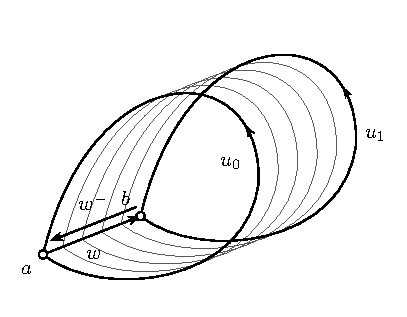
\includegraphics[width=.48\textwidth]{figures/fig04-tikz.pdf}\\图4\end{minipage}\end{center}
\entry{3.14}{定理}
道路连通拓扑空间$X$单连通，当且仅当$X$中任意两条闭曲线作为闭曲线自由同伦。

证明很简单，留给读者。
\entry{3.15}{函子性}
设$f:X\to Y$是拓扑空间之间的连续映射。若$u:I\to X$是$X$中的曲线，则$f\circ u:I\to Y$是$Y$中的曲线。若$u,u':I\to X$同伦，则$f\circ u$与$f\circ u'$也同伦。故$f$诱导基本群之间的映射
\[
f_*:\pi_1(X,a)\longrightarrow\pi_1(Y,f(a)).
\]
这一映射为群同态，因为$f\circ(u\cdot v)=(f\circ u)\cdot(f\circ v)$。若$g:Y\to Z$为另一连续映射，则$(g\circ f)_*=g_*\circ f_*$。
\subsection*{习题（第3节）}
\entry{3.1}{}
(a) 设$X$是流形，$U_1,U_2\subset X$是两个开、连通且单连通的子集，并且$U_1\cap U_2$连通。证明$U_1\cup U_2$单连通。

(b) 利用(a)证明$n\ge2$时$S^n$单连通。
\entry{3.2}{}
设$X,Y$是弧连通拓扑空间。证明$\pi_1(X\times Y)\cong\pi_1(X)\times\pi_1(Y)$。
\sourcepage{20}
\entry{3.3}{}
设$(X,a)$与$(Y,b)$是带基点的拓扑空间，$a\in X$、$b\in Y$。设$f,g:X\to Y$是两个满足$f(a)=g(a)=b$的连续映射。若存在连续映射$F:X\times[0,1]\to Y$，使对每个$x\in X$有$F(x,0)=f(x)$、$F(x,1)=g(x)$，且对每个$t\in[0,1]$有$F(a,t)=b$，则称$f,g$同伦。考虑诱导映射$f_*,g_*:\pi_1(X,a)\to\pi_1(Y,b)$。证明若$f,g$同伦，则$f_*=g_*$。
